% COMPILE: xelatex

\documentclass[a4paper]{article}  % A4 paper size

\usepackage[UTF8]{ctex}  % Chinese support
\usepackage[left=3.17cm, right=3.17cm, top=2.54cm, bottom=2.54cm]{geometry}  % Margins

\usepackage{xcolor}  % Color support
\usepackage{tcolorbox}  % Colored boxes

\usepackage{fancyhdr}  % Header and footer
\usepackage{graphicx, subcaption}  % Figures
\usepackage[shortlabels]{enumitem}  % Enumerate list
\usepackage[sort&compress]{gbt7714}  % Bibliography
\usepackage{hyperref}  % Hyperlinks
\usepackage{booktabs, array}  % Tables
\usepackage{multirow}  % Multirow
\usepackage{amsmath}  % Math

\tcbuselibrary{skins}  % Colored boxes
\tcbuselibrary{minted}  % Code blocks

\setmonofont[]{Fira Code}  % Monospaced font
\usemintedstyle{colorful}  % Code block style set up
\setenumerate{  % Enumerate list set up
    itemsep=0pt,
    partopsep=0pt,
    parsep=\parskip,
    topsep=0pt,
    itemindent=4em,
    leftmargin=0pt,
    listparindent=2em,
    label= (\arabic*)
}
\setitemize{  % Itemize list set up
    itemsep=0pt,
    partopsep=0pt,
    parsep=\parskip,
    topsep=5pt
}
\setdescription{  % Description list set up
    itemsep=0pt,
    partopsep=0pt,
    parsep=\parskip,
    topsep=5pt
}
\hypersetup{  % Hyperlinks set up
    unicode,
    colorlinks=true,
    linkcolor=black,
    urlcolor=black
}


\newtcblisting{codeblock}[2][]{
    listing engine=minted,
    boxrule=0.1mm,
    colback=white!98!black,
    colframe=white!80!black,
    listing only,
    left=5mm,
    enhanced,
    sharp corners=all,
    overlay={
        \begin{tcbclipinterior}
            \fill[white!98!black] (frame.south west) rectangle ([xshift=5mm]frame.north west);
        \end{tcbclipinterior}
    },
    minted language=#2,
    minted style=tango,
    minted options={fontsize=\small,breaklines,autogobble,linenos,numbersep=3mm,escapeinside=\#\#},#1
}


\begin{document}

\title{\textbf{MIPS 32 位流水线处理器设计}\\——夏季学期综合实验报告}
\author{陈子熠}
\date{\today}
\maketitle


\tableofcontents

\newpage

\section{实验目的}

\begin{enumerate}[1]
    \item 学习和理解流水线处理器的设计方法,特别是解决竞争问题的方法(如 forwarding、阻塞、分支和跳转指令处理)。
    \item 扩展对分支指令和跳转指令的理解和实现。
    \item 连接流水线与外设,实现对外设的控制。
    \item 通过软件方式进行译码等操作,体会硬件方式与软件方式的区别。
    \item 通过具体的实验任务,掌握设计、实现、测试和优化处理器的全过程。
    \item 对比和评估流水线 MIPS 处理器与单周期 MIPS 处理器在解决同一问题上的性能差异。
\end{enumerate}


\section{设计方案}

\subsection{总体设计}

\begin{figure}[ht]
    \centering
    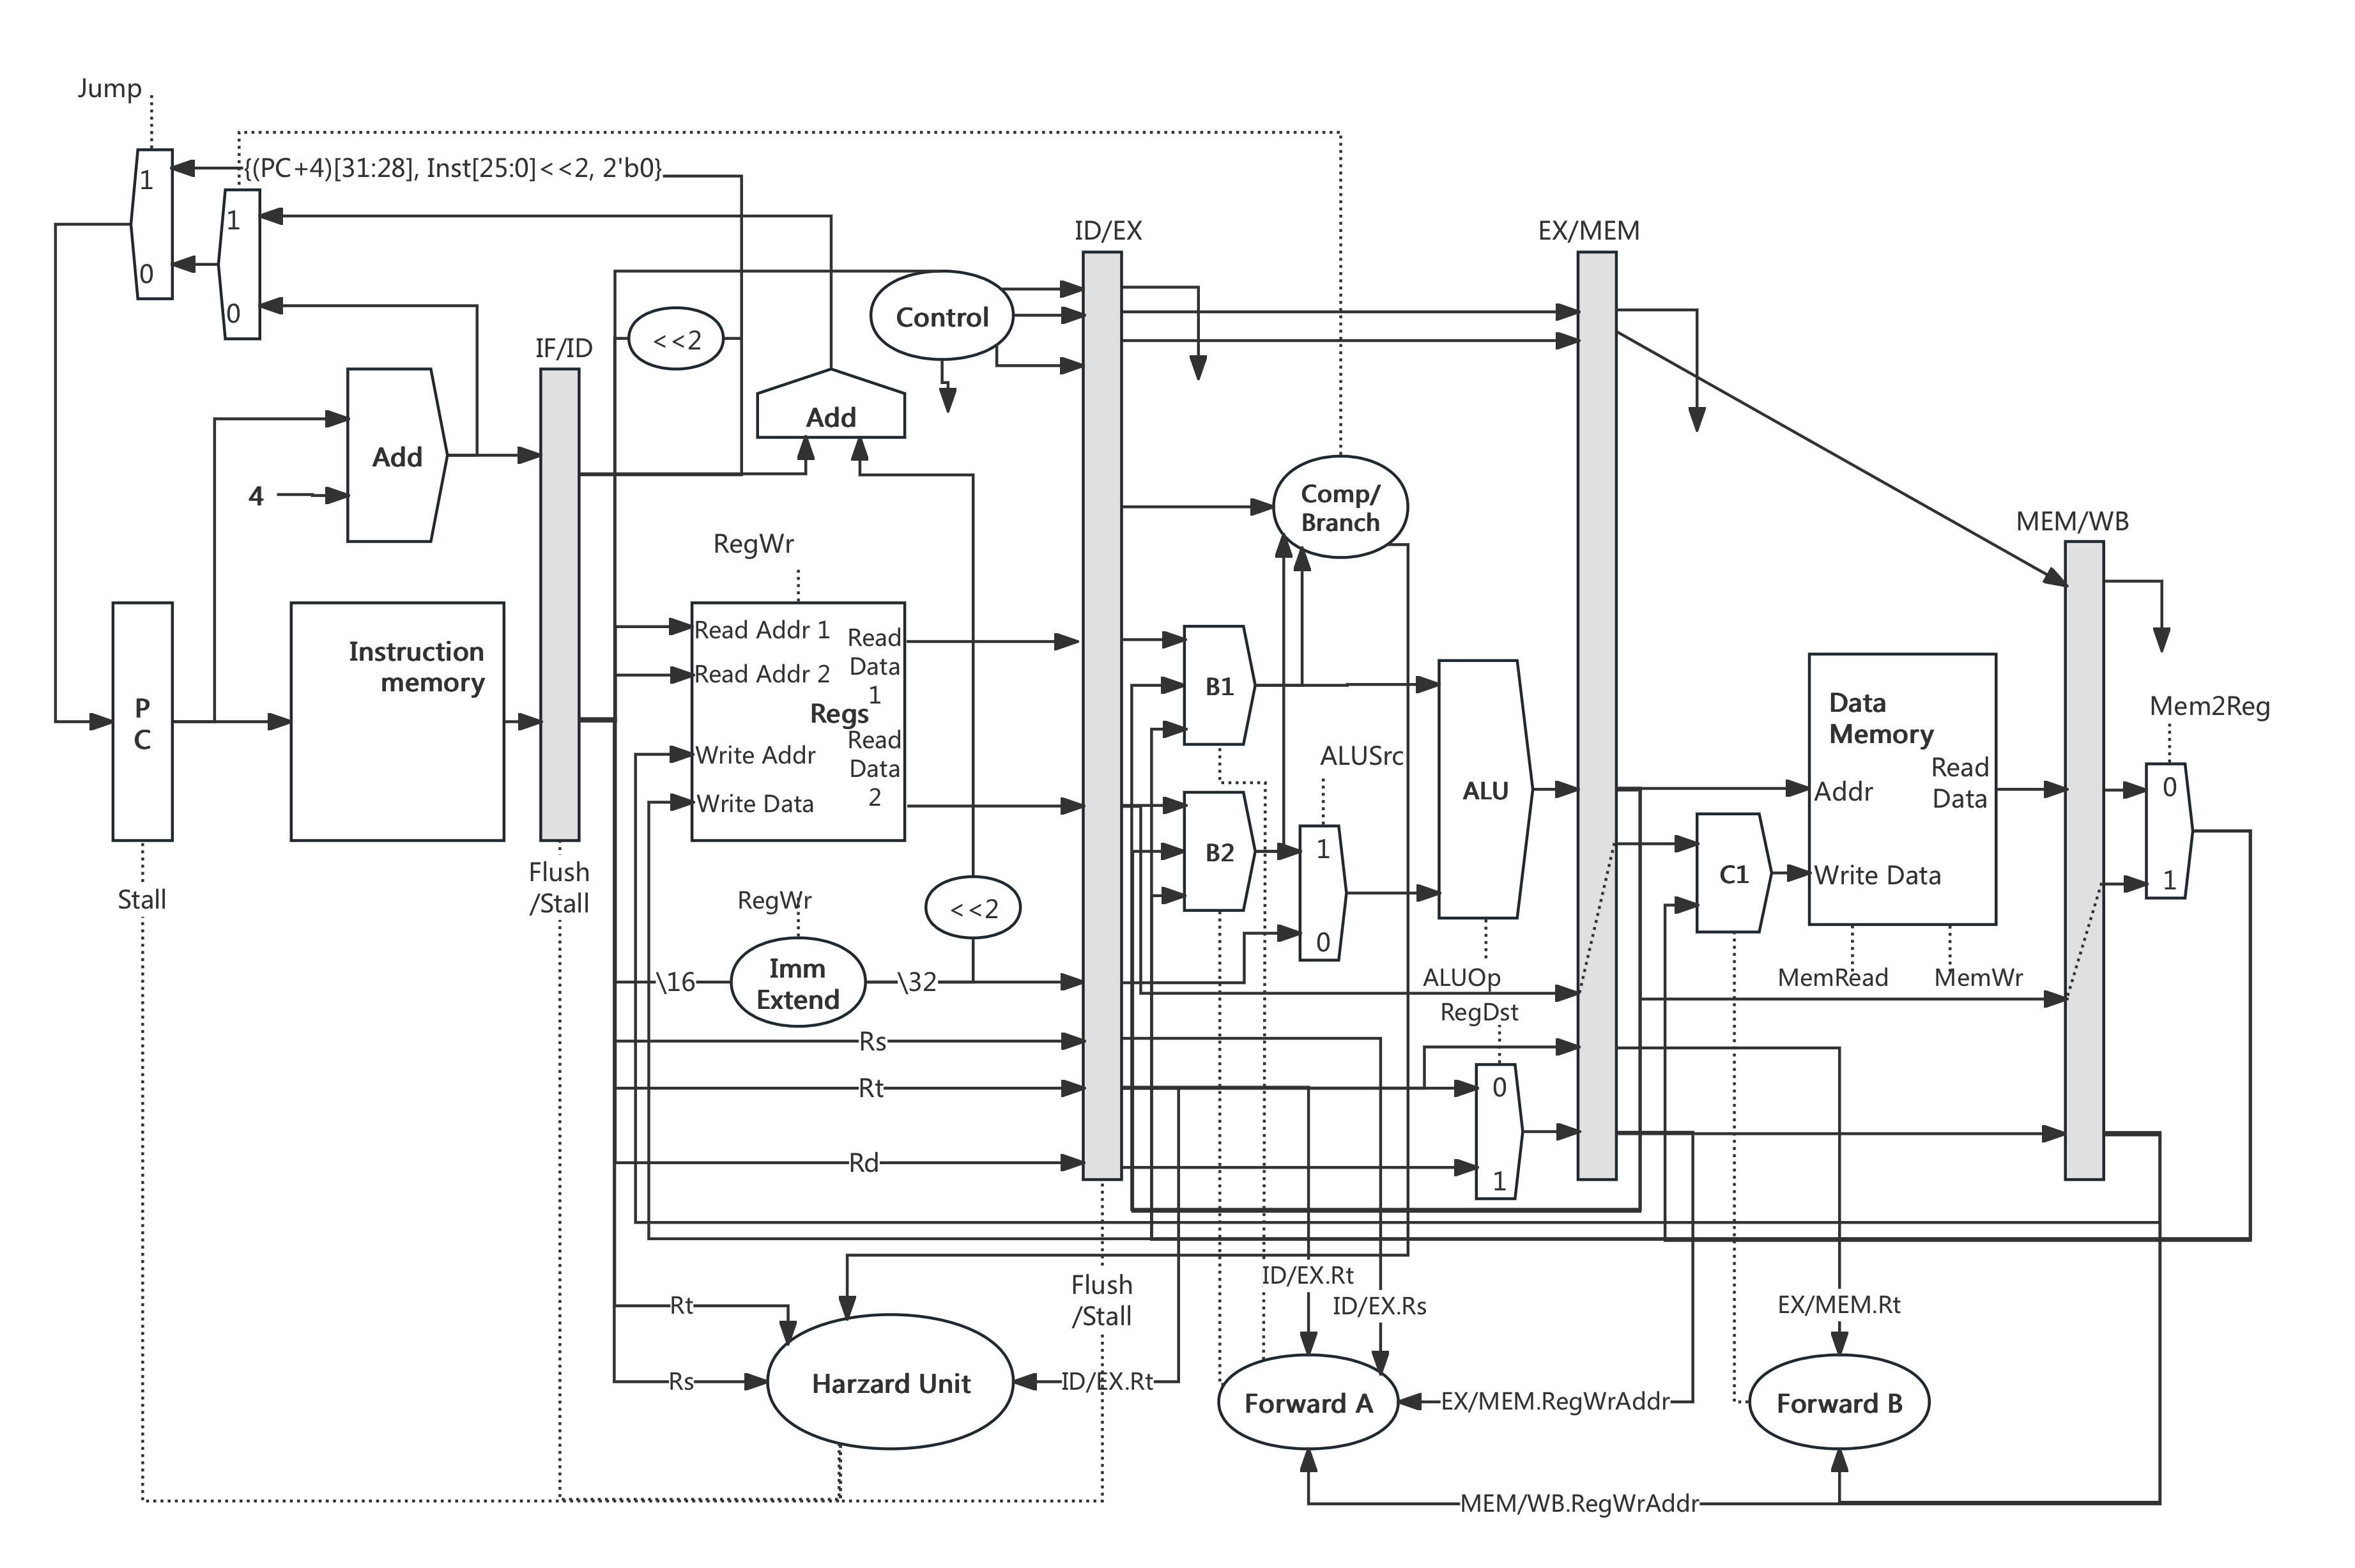
\includegraphics[width=.8\textwidth]{asserts/MIPS32.png}
    \caption{
        MIPS 流水线处理器数据通路
    }\label{fig:pipeline_design}
\end{figure}

本次 MIPS 流水线处理器的数据通路如图 \ref{fig:pipeline_design}。整体设计方案参考了 2024 年清华大学电子工程系《数字逻辑与处理器基础》课件中 5 级流水线的数据通路。在此基础上,进行了如下改进或补充:

\begin{enumerate}[1]
    \item 对于分支指令,采用静态分支预测,默认不发生跳转,以减少 Stall 带来的性能损失。
    \item 在静态分支预测的基础上,将分支指令的判断推迟至 EX 阶段,以降低逻辑复杂度,提高鲁棒性。
    \item J 型指令在 ID 阶段判断,并取消 IF 阶段指令。
    \item 在 Forwarding 电路的基础上增加 Hazard Detection 逻辑,控制级间寄存器的 Stall 与 Flush 操作,用于检测 Forwarding 无法解决的数据冒险问题(如 Load-Use 类竞争)以及处理分支指令带来的控制冒险问题。
    \item 扩充分支指令,如 beq, bne, blez, bgtz, bltz,Opcode 分别为 0x04, 0x05, 0x06, 0x07, 0x01。
    \item 扩充跳转指令,如 j, jal, jr, jalr。其中 j 与 jal 是 J 型指令,Opcode 分别为 0x02, 0x03;jr 与 jalr 是 R 型指令,Funct 分别为 0x08, 0x09。
\end{enumerate}

所支持的指令如下:

\begin{table}[htb]
    \centering
    \caption{
        支持指令
    }\label{tab:instructions}
    \begin{tabular}{cc}
        \toprule
        \textbf{类型} & \textbf{指令} \\
        \midrule
        R 型 & add, addu, sub, subu, mul, and, or, xor, nor, sll, srl, sra, slt, sltu, jr, jalr \\
        I 型 & lw, sw, lui, addi, addiu, andi, slti, sltiu, beq, bne, blez, bgtz, bltz \\
        J 型 & j, jal \\
        \bottomrule
    \end{tabular}
\end{table}
下面将逐一介绍此 MIPS 流水线处理器的设计细节。

\subsection{控制信号}

控制信号基于单周期 MIPS 处理器的设计,并根据流水线的特点进行了调整。
例如,去除了 Branch 控制信号,将分支的判断统一推迟至 EX 阶段,使得分支的判断更简洁优雅;
增加了 bne, blez, bgtz, bltz 等分支指令的控制信号,以支持更多的分支指令;
增加了 jalr 等指令的控制信号,以支持更多的跳转指令。
具体的控制信号见附录图\ref{adx:control_signals}。

\subsection{Forward Unit}

Forward Unit 用于解决数据冒险以及控制冒险问题,主要包括 EX/MEM 级间寄存器至 EX 阶段的数据转发和 MEM/WB 级间寄存器至 EX、MEM 阶段的数据转发。伪代码如下:

\begin{codeblock}{verilog}
    // EX Forwarding
    if (EX/MEM.RegWr && EX/MEM.RegWrAddr != 0 && EX/MEM.RegWrAddr == ID/EX.RxAddr) {
        Forward = 2'b01;
    } else if (MEM/WB.RegWr && MEM/WB.RegWrAddr != 0 && MEM/WB.RegWrAddr == ID/EX.RxAddr) {
        Forward = 2'b10;
    } else {
        Forward = 2'b00;
    }
    // MEM Forwarding
    if (MEM/WB.RegWr && MEM/WB.RegWrAddr != 0 && MEM/WB.RegWrAddr == EX/MEM.RtAddr) {
        Forward = 1'b1;
    } else {
        Forward = 1'b0;
    }
\end{codeblock}

值得注意的是,控制冒险解决方案中的 Forwarding 电路与数据冒险解决方案中到达 EX 阶段的 Forwarding 电路逻辑完全一致,故可直接复用。

\subsection{Hazard Unit}

Hazard Unit 用于检测 Forwarding 无法解决的数据冒险问题(如 Load-Use 类竞争)以及处理分支指令带来的控制冒险问题,生成 Stall 与 Flush 控制信号。

\subsubsection{Load-Use 竞争}

Load-Use 竞争是指在 Load 指令的 MEM 阶段写回数据到寄存器之前,后续的指令需要读取该寄存器的数据,导致数据冒险。
为了解决 Load-Use 竞争,需要在 ID 阶段检测到竞争后,Stall IF/ID 级间寄存器并 Flush ID/EX 级间寄存器。

值得注意的是,对于 Load-Store 类竞争,并不需要进行额外的 Stall 操作。
相反,该类竞争可被 Forwarding 电路自动解决,而 Stall 操作的使用反而容易导致逻辑冲突。
这一点在课件 Hazard 一章中并未提及。伪代码如下:

\begin{codeblock}{verilog}
    if (ID/EX.MemRd && (ID/EX.RtAddr == IF/ID.RsAddr || ID/EX.RtAddr == IF/ID.RtAddr) && !IF/ID.MemWr) {
        IF/ID.Stall = 1'b1;
        ID/EX.Flush = 1'b1;
    }
\end{codeblock}

\subsubsection{分支指令}
分支指令采用静态分支预测技术,并在 EX 阶段判断是否发生跳转。
若发生跳转,则需要 Flush IF/ID 与 ID/EX 级间寄存器,并 Stall PC 寄存器。
伪代码如下:(注意这里的 Branch 控制信号代表是 Branch 指令且需要跳转)

\begin{codeblock}{verilog}
    if (Branch) {
        IF/ID.Flush = 1'b1;
        ID/EX.Flush = 1'b1;
        PC.Stall = 1'b1;
    }
\end{codeblock}

\subsubsection{跳转指令}

对于 J 型指令 j, jal,需要在 ID 阶段判断是否发生跳转。
若发生跳转,则需要 Flush IF/ID 级间寄存器,并更新 PC 寄存器。

对于 R 型指令 jr, jalr,则在 EX 阶段判断是否发生跳转,以最大程度地复用 EX 阶段的 Forwarding 电路。
若发生跳转,则需要 Flush IF/ID 与 ID/EX 级间寄存器,并更新 PC 寄存器。

由于 J 型指令占比较小,所引入 Stall 的影响可以忽略不计。
具体逻辑实现与分支指令类似,故不再赘述。

\subsection{存储器}

存储器采用哈佛架构,数据存储器与指令存储器分离。
其中数据存储器采用双端口 RAM,指令存储器采用单端口 ROM。

数据存储器的地址空间被划分为两个部分:

\begin{enumerate}[A]
    \item 0x00000000 - 0x3FFFFFFF 为数据 RAM,提供数据存储功能。
    \item 0x40000000 - 0x7FFFFFFF 为外设地址空间,对其地址的读写对应到相应的外设资源。
\end{enumerate}

由于硬件资源受限,数据 RAM 的大小被限制在 512 个 32 位字。
外设地址空间的有效地址包括 0x40000010, 0x40000018, 0x4000001C 与 0x40000020,分别对应于七段数码管、串口发送数据(UART\_TXD)、串口接收数据(UART\_RXD)与串口状态控制(UART\_CON)。

\subsection{外设}

外设均采用软件方式译码,通过对外设地址空间的读写实现对外设的控制。

\subsubsection{LED}

LED 通过对外设地址 0x40000010 的写入实现对 LED 灯的控制。
0x40000010 地址的低 7 位对应于 7 个 LED 灯的状态,第 7 位对应于小数点,8-11 位对应于 4 个数码管的使能。
该地址的内容被直接转发到 LED 灯的控制端口,实现对 LED 灯的控制。

显示时,利用人眼视觉暂留效应,使用软件延时,每位显示1ms,轮流显示各位数字,实现动态显示效果。

\subsubsection{UART}

UART 的 RX 与 TX 模块直接复用了实验 3 的设计。
通过检测地址 0x40000020(对应 UART\_CON)的数据,可以检查串口的发送/接收状态,实现用软件方式控制串口的发送与接收。

从串口接收数据时,通过检测地址 0x40000020 的第 3 位,可确定接收缓冲区是否为空。
若为空,则等待串口接收数据;若不为空,则读取地址 0x4000001C(对应 UART\_RXD)的数据,即可获取串口接收到的数据。

向串口发送数据时,向地址 0x40000018(对应 UART\_TXD)写入数据即可触发数据的发送。
通过检测地址 0x40000020 的第 2 位,可确定发送是否完成。若发送未完成,则等待串口发送数据;若发送完成,则可继续发送下一组数据。

由于串口每次只能发送一个字节的数据,故需要在发送或接收数据时需要将 32 位的数据通过移位的方式拆分为 4 个字节进行发送或接收。

\section{文件清单}

源代码位于 src 目录下。锁相环分频器由 Vivado IP core 直接生成。文件结构及说明如下:

\begin{codeblock}{bash}
    src
    |-- config
    |   `-- CPU.xdc  # 约束文件
    |-- source
    |   |-- ALU.v       # 算术逻辑单元
    |   |-- ALU_Ctrl.v  # ALU 控制单元
    |   |-- Branch.v    # 分支控制单元
    |   |-- CPU.v       # CPU 顶层模块
    |   |-- Ctrl.v      # 控制单元
    |   |-- Data_Mem.v  # 数据存储器,包括 RAM 与外设
    |   |-- EX_MEM.v    # EX/MEM 级间寄存器
    |   |-- Forward.v   # Forwarding 单元
    |   |-- ID_EX.v     # ID/EX 级间寄存器
    |   |-- IF_ID.v     # IF/ID 级间寄存器
    |   |-- Inst_Mem.v  # 指令存储器
    |   |-- MEM_WB.v    # MEM/WB 级间寄存器
    |   |-- PC.v        # PC 寄存器
    |   |-- RF.v        # 寄存器堆
    |   `-- UART
    |       |-- UART_RX.v  # 串口接收模块
    |       `-- UART_TX.v  # 串口发送模块
    `-- test
        |-- Test_CPU.v  # CPU 测试文件
        `-- asm
            |-- binary_insert_sort.asm        # 二分插入排序汇编代码
            |-- binary_insert_sort.hex        # 二分插入排序机器码
            |-- binary_insert_sort.inst       # 二分插入排序指令
            |-- binary_insert_sort_uart.asm   # 二分插入排序汇编代码(含串口通信)
            |-- binary_insert_sort_uart.hex   # 二分插入排序机器码(含串口通信)
            |-- binary_insert_sort_uart.inst  # 二分插入排序指令(含串口通信)
            |-- data.bin                      # 测试数据原始二进制文件
            |-- data.hex                      # 测试数据十六进制文件
            |-- data.inst                     # 测试数据指令文件(仅用于不含串口通信的测试)
            |-- data.txt                      # 测试数据十进制文本文件
            `-- script
                |-- bin_reader.cpp                   # 二进制文件读取工具
                |-- binary_insert_sort_runnable.asm  # 二分插入排序汇编代码(含文件读写,可运行)
                |-- data_generator.py                # 测试数据生成工具
                |-- inst_generator.py                # 指令生成工具
                `-- load_file_runnable.asm           # 文件读写汇编代码(可运行)
\end{codeblock}

\section{关键代码}

\subsection{寄存器的先写后读}

寄存器采用先写后读的方式,有效解决了部分数据冒险问题,提高了流水线的效率。关键代码如下:

\begin{codeblock}{verilog}
assign RdData1 = RsAddr == 0 ? 32'h00000000 :
                 RegWr && WrAddr == RsAddr ? WrData :
                 RF_data[RsAddr];
assign RdData2 = RtAddr == 0 ? 32'h00000000 :
                 RegWr && WrAddr == RtAddr ? WrData :
                 RF_data[RtAddr];
\end{codeblock}

\subsection{Forwarding 控制单元}

用于处理数据冒险和控制冒险问题,减少 Stall,提高流水线的效率。关键代码如下:

\begin{codeblock}{verilog}
assign EX_ForwardRs = 
                (EX_MEM_RegWr && EX_MEM_RegWrAddr != 0 && EX_MEM_RegWrAddr == ID_EX_RsAddr) ? 2'b01 :  // EX/MEM to EX
                (MEM_WB_RegWr && MEM_WB_RegWrAddr != 0 && MEM_WB_RegWrAddr == ID_EX_RsAddr) ? 2'b10 :  // MEM/WB to EX
                2'b00;
assign EX_ForwardRt = 
                (EX_MEM_RegWr && EX_MEM_RegWrAddr != 0 && EX_MEM_RegWrAddr == ID_EX_RtAddr) ? 2'b01 :  // EX/MEM to EX
                (MEM_WB_RegWr && MEM_WB_RegWrAddr != 0 && MEM_WB_RegWrAddr == ID_EX_RtAddr) ? 2'b10 :  // MEM/WB to EX
                2'b00;
assign MEM_ForwardRt = 
                (MEM_WB_RegWr && MEM_WB_RegWrAddr != 0 && MEM_WB_RegWrAddr == EX_MEM_RtAddr) ? 1'b1 :  // MEM/WB to MEM
                1'b0;
\end{codeblock}

\subsection{Hazard 检测单元}

用于检测 Forwarding 无法解决的数据冒险问题(如 Load-Use 类竞争)以及处理分支指令带来的控制冒险问题,生成 Stall 与 Flush 控制信号。关键代码如下:

\begin{codeblock}{verilog}
assign LdUseHazard = 
                (ID_EX_MemRd && (ID_EX_RtAddr == IF_ID_RsAddr || ID_EX_RtAddr == IF_ID_RtAddr) && !MemWr) ? 1'b1 :
                1'b0;
assign IF_ID_HzCtrl = 
                (Branch || ID_EX_PCSrc == 2'b10 || PCSrc == 2'b01) ? 2'b01 :  // branch or jump register or jump hazard, flush
                LdUseHazard ? 2'b10 :  // load-use hazard, stall
                2'b00;  // normal
assign ID_EX_HzCtrl = 
                (Branch || LdUseHazard || ID_EX_PCSrc == 2'b10) ? 2'b01 :  // branch or load-use or jump register hazard, flush
                2'b00;  // normal
\end{codeblock}

\subsection{级间寄存器的刷写}

在检测到数据冒险或控制冒险时,需要 Flush 或 Stall IF/ID 与 ID/EX 级间寄存器,以清空流水线中的指令。关键代码如下:

\begin{codeblock}{verilog}
always @(posedge clk or posedge rst) begin
    if (rst) begin
        IF_ID_RsAddr <= 5'h00;
        ...
    end
    else begin
        if (HzCtrl == 2'b01) begin  // Flush
            IF_ID_RsAddr <= 5'h00;
            ...
        end
        else if (HzCtrl == 2'b00) begin  // Normal
            IF_ID_RsAddr <= Inst[25:21];
            ...
        end
        // Else Stall, do nothing
    end
end
\end{codeblock}

\subsection{分支控制单元}

分支控制单元用于判断分支指令是否发生跳转,以及跳转的目标地址。关键代码如下:

\begin{codeblock}{verilog}
// Branch is 1 if and only if the branch instruction is executed and the branch condition is satisfied
assign Branch =
            (OpCode == 6'h04 && RsData == RtData) ? 1'b1:  // beq
            (OpCode == 6'h05 && RsData != RtData) ? 1'b1:  // bne
            (OpCode == 6'h06 && RsData <= 32'd0) ? 1'b1:  // blez
            (OpCode == 6'h07 && RsData > 32'd0) ? 1'b1:  // bgtz
            (OpCode == 6'h01 && RsData < 32'd0) ? 1'b1:  // bltz
            1'b0;
\end{codeblock}

\subsection{堆栈操作的实现}

为支持二分插入排序算法,需要支持堆栈操作。本次实验中,由于数据量不大,可以最大化利用已有数据存储器,将堆栈空间设置在数据存储器有效存储空间的高地址空间(0x000007FF 及以下)。关键代码如下:

\begin{codeblock}{verilog}
always @(posedge clk or posedge rst) begin
    if (rst) begin
        for (i = 1; i < 29; i = i + 1)
            RF_data[i] = 32'h00000000;
        RF_data[29] = 32'h000007FF;
        ...
    end
    else ...
end
\end{codeblock}

\subsection{外设连接}

外设连接通过软件方式实现,通过对外设地址空间的读写实现对外设的控制。关键代码如下:

\begin{codeblock}{verilog}
// Read data
assign RdData = 
            MemRd ? (
                Addr == 32'h4000001C ? {24'h0, RxByte} :  // UART_RXD
                Addr == 32'h40000020 ? {27'h0, UART_Ctrl, 2'b0} :  // UART_CON
                Addr == 32'h40000018 ? 32'h00000000 :  // UART_TXD, write only
                RAM_Data[AddrWord]  // RAM
            ) : 32'h00000000;  // default
always @(posedge clk or posedge rst) begin
    if (MemRd && Addr == 32'h40000020)  // Auto flush UART_Ctrl if read
        UART_Ctrl[1:0] <= 2'b00;
end
\end{codeblock}

\begin{codeblock}{verilog}
// Write data
always @(posedge clk or posedge rst) begin
    if (rst) ...
    else begin
        if (MemWr) begin
            if (Addr == 32'h40000010)  // LED
                RAM_Digi <= WrData[11:0];
            else if (Addr == 32'h40000018) begin  // UART_TXD
                TxByte <= WrData[7:0];
                TxValid <= 1'b1;
            end
            else if (Addr[31:2] < RAM_SIZE)  // RAM
                RAM_Data[AddrWord] <= WrData;
        end
        ...
    end
end
\end{codeblock}

\section{算法指令}

\subsection{BCD 译码}

利用汇编指令将 16 进制数转换为对应 BCD 码,以便在七段数码管上显示。采用内存地址映射的方式,给定 16 进制数字,通过读取对应地址的数据,即可获取对应的 BCD 码。关键代码如下:

\begin{codeblock}{ASM}
li $s0, 2047  # 0x000007FF
li $t0, 63  # Digit 0
sw $t0, 0($s0)
li $t0, 6  # Digit 1
sw $t0, -4($s0)
...
li $t0, 113  # Digit F
sw $t0, -60($s0)
\end{codeblock}

\subsection{BCD 显示延时}

BCD 显示延时汇编指令用于实现动态显示 BCD 码。通过软件延时,每次显示一个数码管,利用人眼视觉暂留效应,实现动态显示效果。关键代码如下:

\begin{codeblock}{ASM}
# stall, f0=75MHz, f=1KHz, stall=75KT, 5T per loop
stall_10k:
li $t2, 15000
stall_10k_loop:
subi $t2, $t2, 1
bne $t2, $zero, stall_10k_loop
jr $ra
\end{codeblock}

\subsection{UART 接收数据}

UART 接收数据汇编指令用于从串口接收数据。通过检测串口状态,若接收缓冲区非空,则读取接收数据。4 个字节的数据通过移位的方式合并为 32 位数据。由于第一个 32 位数据表示数据长度,可根据该数据判断需要接收的总数据量。关键代码如下:

\begin{codeblock}{ASM}
li $s0, 1073741848  # 0x40000018
jal receive_wait_loop  # Wait for 4 most significant bits
lw $t1, 4($s0)
sll $t1, $t1, 24
jal receive_wait_loop # Wait for data 4 second most significant bits
lw $t2, 4($s0)
sll $t2, $t2, 16
or $t2, $t1, $t2  # concat $t1, $t2
... # Similar for $t3, $t4
sw $t4, 0($a0)  # Store 32 bits data
\end{codeblock}

\subsection{UART 接收忙等待}

采用忙等待的方式等待串口接收数据。通过检测串口状态,若接收缓冲区非空,则退出等待。关键代码如下:

\begin{codeblock}
receive_wait_loop:
lw $t0, 8($s0)
sll $t0, $t0, 28  # RxDone
srl $t0, $t0, 31
beq $t0, $zero, receive_wait_loop
jr $ra
\end{codeblock}

\subsection{UART 发送数据}

UART 发送数据汇编指令用于向串口发送数据。首先通过移位的方式将 32 位数据拆分为 4 个字节,然后通过串口发送数据。关键代码如下:

\begin{codeblock}{ASM}
lw $t0, 0($a0)  # $a0 is where data is stored
srl $t1, $t0, 24  # $t1 = $t0[31:24]
sll $t2, $t0, 8  # $t2 = $t0[23:16]
srl $t2, $t2, 24
... # Similar for $t3, $t4
sw $t1, 0($s0)
jal send_wait_loop
sw $t2, 0($s0)
jal send_wait_loop
... # Similar for $t3, $t4
\end{codeblock}

\subsection{UART 发送忙等待}

采用忙等待的方式等待串口发送数据。通过检测串口状态,若发送完成,则退出等待。关键代码如下:

\begin{codeblock}{ASM}
send_wait_loop:
lw $t0, 8($s0)  # TxDone
sll $t0, $t0, 29
srl $t0, $t0, 31
beq $t0, $zero, send_wait_loop
jr $ra
\end{codeblock}

\subsection{指令生成}

此脚本用于将机器码转换为汇编指令,以降低人力成本,方便测试。关键代码如下:

\begin{codeblock}{python}
def read_instructions(file_path):  # Read machine code from file
    with open(file_path, 'r') as file:
        lines = file.readlines()
    return [line.strip() for line in lines]

def format_instructions(instructions):  # Format machine code to instructions
    formatted_lines = []
    for i, instruction in enumerate(instructions):
        formatted_line = f"9'd{i}: Inst <= 32'h{instruction};"
        formatted_lines.append(formatted_line)
    return formatted_lines

def write_formatted_instructions(file_path, formatted_lines):  # Write formatted instructions to file
    with open(file_path, 'w') as file:
        for line in formatted_lines:
            file.write(line + '\n')
\end{codeblock}

\section{仿真结果}

\subsection{数据准备}

测试数据复用了汇编大作业的测试数据,包含 21 个 32 位数据,用于测试排序算法。
其中排序前第一个数据表示数据量,排序后第一个数据表示比较次数,由汇编大作业的排序算法计算得出。

\begin{table}[htb]
    \centering
    \caption{
        测试数据
    }\label{tab:test_data}
    \begin{tabular}{{cp{12.5cm}}}
        \toprule
        \textbf{排序前} & 00 14, 41 A8, 3A F2, AC DA, 0C 2B, B7 83, DA C9, 8E D9, 09 FF, 2F 44, 04 4E, 98 99, 3C 56, 12 8D, DB E3, D4 B4, 37 48, 39 18, 41 12, C3 99, 49 55 \\
        \midrule
        \textbf{排序后} & 00 3E, 04 4E, 09 FF, 0C 2B, 12 8D, 2F 44, 37 48, 39 18, 3A F2, 3C 56, 41 12, 41 A8, 49 55, 8E D9, 98 99, AC DA, B7 83, C3 99, D4 B4, DA C9, DB E3 \\
        \bottomrule
    \end{tabular}
\end{table}

\subsection{排序仿真}

为快速测试排序的准确性,我们在指令中去除了串口通信的部分,保留排序与显示部分。
在这种情况下,测试数据通过 python 脚本格式化为 verilog 语言初始化在数据存储器中。
仿真结果如图\ref{fig:simulation_sort}所示。

\begin{figure}[ht]
    \centering
    \begin{subfigure}[b]{0.48\textwidth}
        \centering
        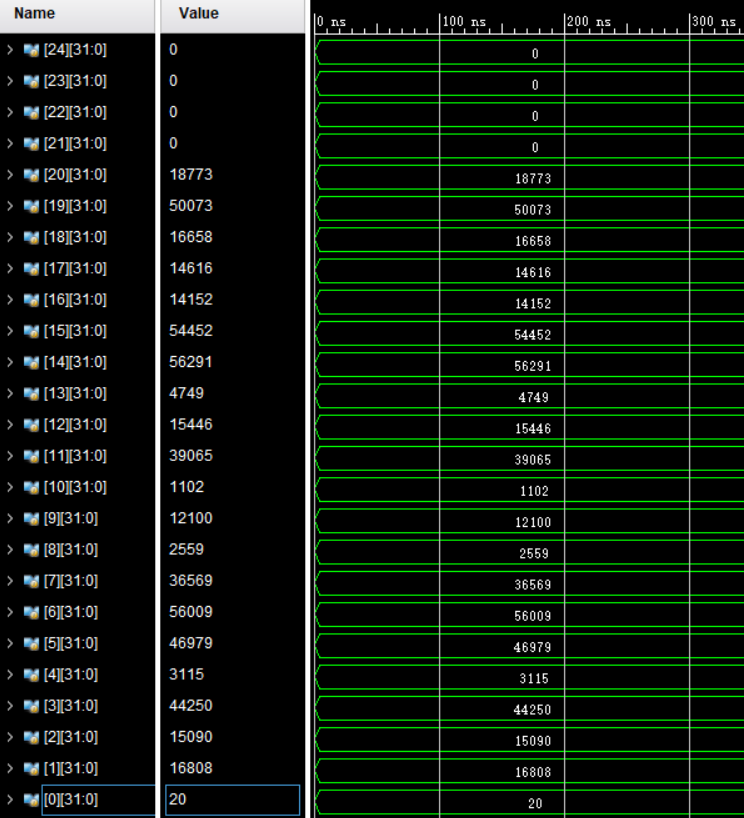
\includegraphics[width=\textwidth]{asserts/data_origin.png}
    \end{subfigure}
    \hfill
    \begin{subfigure}[b]{0.48\textwidth}
        \centering
        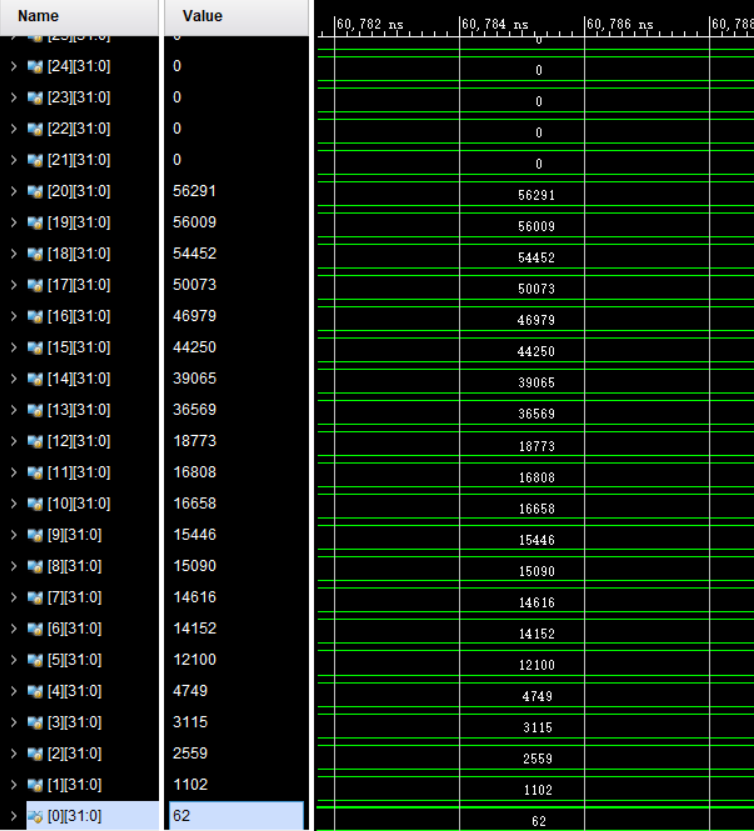
\includegraphics[width=\textwidth]{asserts/data_sort.png}
    \end{subfigure}
    \caption{
        左:排序前,第一个数据表示数据量 \\
        右:排序后,第一个数据表示比较次数
    }\label{fig:simulation_sort}
\end{figure}

可见,排序算法在仿真中得到了正确的结果,从而初步验证了 MIPS 流水线处理器功能的正确性。

\subsection{CPI 计算}

通过 MARS 运行二分插入排序可执行代码,计算指令数,结果如图\ref{fig:instruction_count_sort}所示。

\begin{figure}[ht]
    \centering
    \begin{subfigure}[b]{0.45\textwidth}
        \centering
        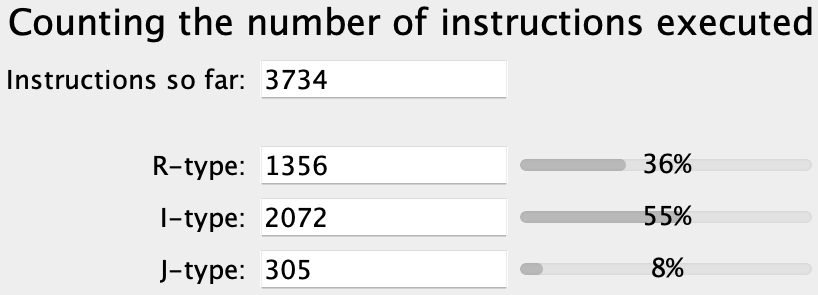
\includegraphics[width=\textwidth]{asserts/instruction_count_sort.png}
        \caption{
            排序总指令数
        }\label{fig:instruction_count_sort}
    \end{subfigure}
    \hfill
    \begin{subfigure}[b]{0.45\textwidth}
        \centering
        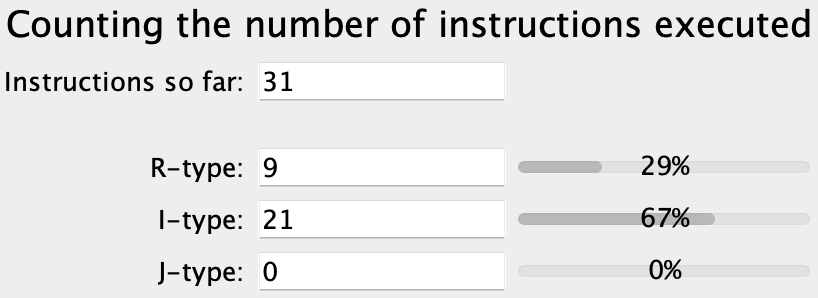
\includegraphics[width=\textwidth]{asserts/instruction_count_io.png}
        \caption{
            文件读写指令数
        }\label{fig:instruction_count_io}
    \end{subfigure}
    \caption{
        左:排序前,第一个数据表示数据量 \\
        右:排序后,第一个数据表示比较次数
    }\label{fig:instruction_count}
\end{figure}

由于该可执行程序存在文件读写操作,所得指令数相比实际排序指令数偏多。

为解决这个问题,将排序过程去除后再次计算指令数,用含排序的指令数减去不含排序的指令数,即可抵消文件读写操作带来的误差,得到实际排序指令数。
不含排序的指令书计算结果如图\ref{fig:instruction_count_io}所示,约 31 条。

根据测试用汇编代码可知,从初始化完成到 LED 开始显示,可近似为排序算法消耗的时间 + 加载 LED 内存地址映射所需时间,后者指令数约为 34 条,恰与文件读写操作执行数相仿。
这意味着两者产生的误差相互抵消。因此可直接用从初始化完成到 LED 开始显示的时间除以排序总指令数较准确地计算得到 CPI。

仿真从初始化完成到 LED 开始显示用时如图\ref{fig:time_consumption}所示,约为 59773ns。

\begin{figure}[ht]
    \centering
    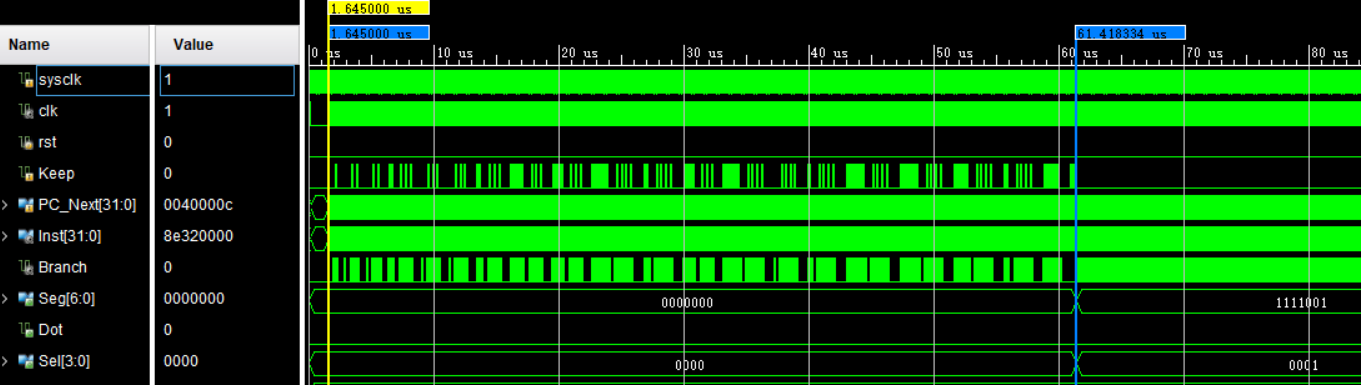
\includegraphics[width=.95\textwidth]{asserts/time_consumption.png}
    \caption{
        排序算法消耗时间
    }\label{fig:time_consumption}
\end{figure}

仿真时,采用时钟频率为 75MHz,故总时钟数为

\begin{align}
    \text{Total Clocks} &= 59773 \times 75 \times 10^{-3} \approx 4483
\end{align}

故 CPI 为

\begin{align}
    \text{CPI} &= \frac{4483}{3734} \approx 1.20
\end{align}

事实上,由于采用静态分支预测,实际 CPI 可能会因分支预测错误率不同而有所浮动。

\subsection{LED 显示仿真}

完成排序算法后,将自动开始动态显示排序后的数据。仿真结果如图\ref{fig:simulation_led}所示。

\begin{figure}[ht]
    \centering
    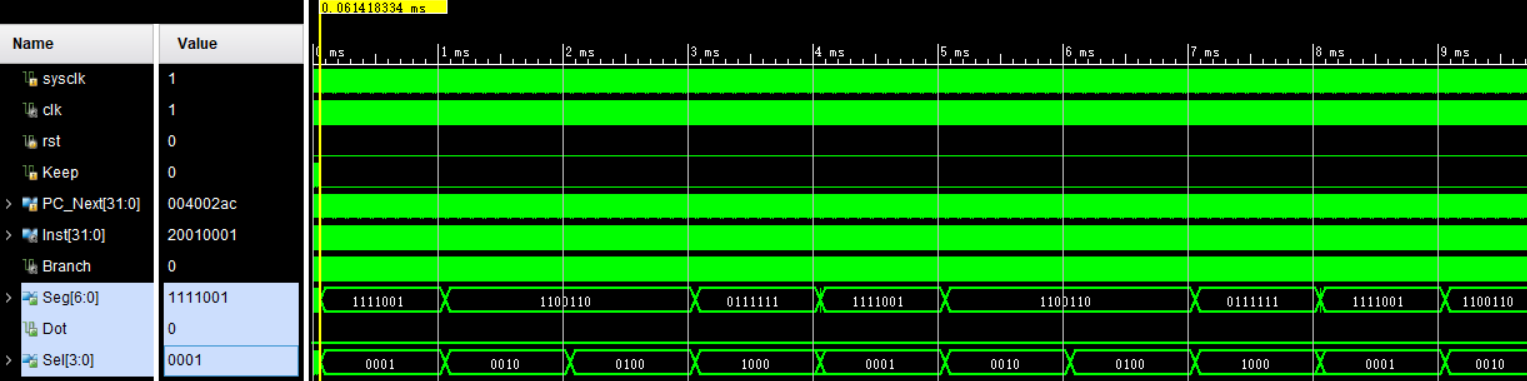
\includegraphics[width=.95\textwidth]{asserts/led.png}
    \caption{
        LED 显示仿真
    }\label{fig:simulation_led}
\end{figure}

可见,使能信号依次为 1, 2, 4, 8;第一个排序后有效数据 0x044E 得到了正确的 BCD 码显示(从低位至高位扫描),从而初步验证了 LED 外设的正确性。

\section{综合情况}

\subsection{资源占用}

综合后资源占用情况如图\ref{fig:utilization_hierarchy}与图\ref{fig:utilization_summary}所示。

\begin{figure}[ht]
    \centering
    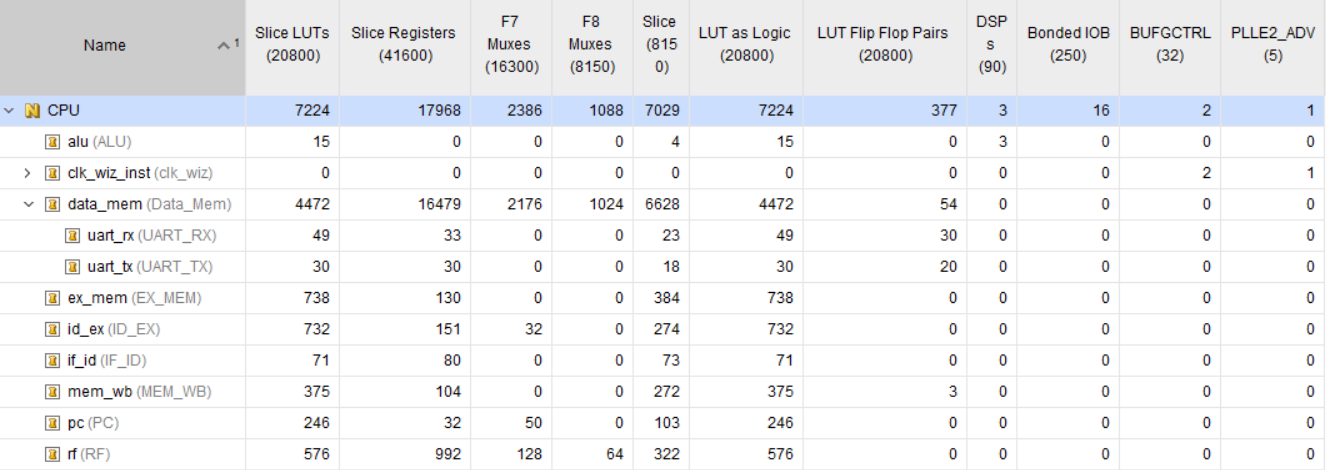
\includegraphics[width=.9\textwidth]{asserts/utilization_hierarchy.png}
    \caption{
        资源占用
    }\label{fig:utilization_hierarchy}
\end{figure}

\begin{figure}[ht]
    \centering
    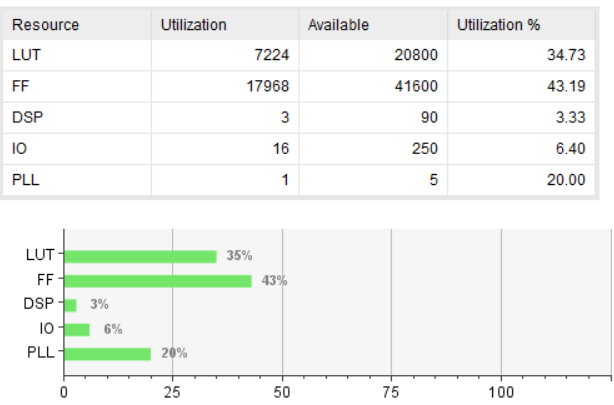
\includegraphics[width=.6\textwidth]{asserts/utilization_summary.png}
    \caption{
        资源占比
    }\label{fig:utilization_summary}
\end{figure}

可见,绝大部分资源为存储器所占用,去除存储器(保留 UART 模块)后,LUT 约为 2831 个,FF 约为 1552 个,DSP 3 个。

与单周期处理器相比(LUT 748 个,FF 201 个,DSP 3 个),流水线处理器的资源占用大大增加。
主要原因可能在于流水线转发等控制逻辑相比单周期处理器大大增加,同时级间寄存器的引入也大幅增加了资源占用。

此外,尽管存储器占用了大量资源,但资源占用率仍然不到一半,去除存储器后仅占用了 10\% 左右的资源,可见 FPGA 拥有的资源容量在教学场景下具有较大的余量。

\subsection{静态时序分析}

综合后静态时序分析结果如图\ref{fig:time_summary}所示,所用时钟如图\ref{fig:clock_summary}所示。

\begin{figure}[ht]
    \centering
    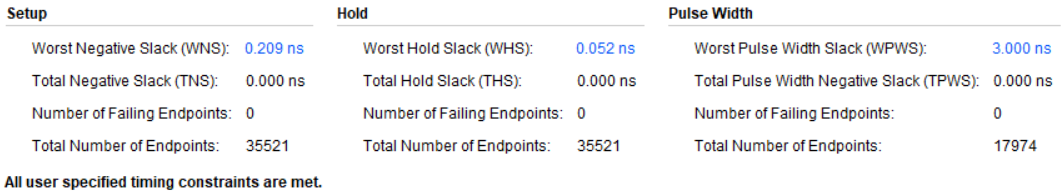
\includegraphics[width=.9\textwidth]{asserts/time_summary.png}
    \caption{
        时序分析
    }\label{fig:time_summary}
\end{figure}

\begin{figure}[ht]
    \centering
    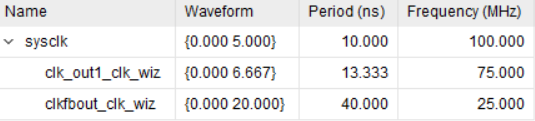
\includegraphics[width=.6\textwidth]{asserts/clock_summary.png}
    \caption{
        时钟
    }\label{fig:clock_summary}
\end{figure}

实际利用锁相环生成的时钟频率为 75MHz,建立时间裕量为 0.209ns,最大时钟频率可达到 76.20MHz(计算过程如下)

\begin{align}
    f_{\text{max}} &= \frac{1}{\text{实际时钟周期-建立时间裕量}} \\
    &= \frac{1}{13.333-0.209}\times 10^9 \\
    &= 76.20 \text{MHz}
\end{align}

\section{硬件调试情况}

\subsection{LED 显示}

该部分已通过助教验收。由于报告中不方便展示 LED 显示效果,故不详细展开。

\subsection{UART 通信}

UART 通信部分已通过助教验收。串口调试助手收发截图如图\ref{fig:uart_result}所示。

\begin{figure}[ht]
    \centering
    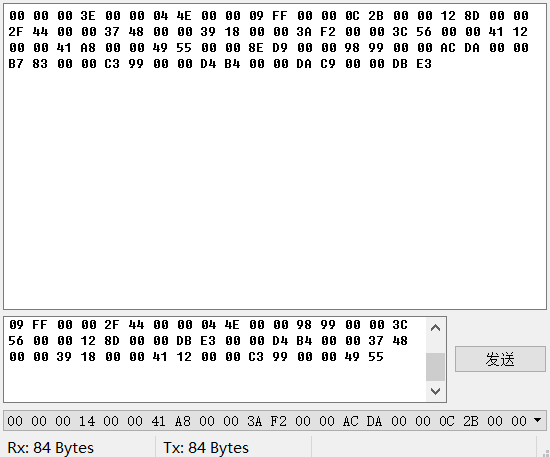
\includegraphics[width=.7\textwidth]{asserts/uart_result.png}
    \caption{
        UART 通信结果
    }\label{fig:uart_result}
\end{figure}

可见结果与表\ref{tab:test_data}中的理论排序后结果一致,从而验证了 UART 通信的正确性。

\section{思想体会}

本次实验中,起初对流水线的设计与 DEBUG 过程较为顺利,在预期的时间内通过了仿真对排序与 LED 显示的验证(耗时共约 10 小时)。
然而,在之后的几天时间里,在烧板子环节遇到了极大的困难。行为仿真可以通过,但在板子上运行时,LED 无法正常显示,令我百思不得其解。
3 天后,在老师和助教的帮助下,终于发现了问题所在(此过程时间跨度极长,具体耗时难以估计)。
之后的 UART 通信由于已有实验 3 以及 LED 软件方法显示的基础,很快完成了整个实验。

下面,将详细描述在烧板子过程中遇到的问题以及解决方法。

起初,我认为问题可能出在板子上。然而,在尝试与舍友交换板子后,问题依然存在,排除了板子硬件问题。

之后,我将问题聚焦在约束文件上。经过与舍友讨论,我们一致认为约束文件应该没有问题。

那么,问题究竟出在哪里呢?那时的我天真地以为,既然仿真能够通过,那么便无法从仿真结果中找到问题所在,于是像个无头苍蝇一样天马行空地寻找问题。

例如,我注意到了综合后生成的一个警告,认为是时钟未正确生成导致的。然而,经过与助教讨论、与助教一起上网查找资料以及在线询问老师后,我们发现这个警告并不是问题的根源。

再如,我认为问题可能出在电脑的 Vivado 环境上。我尝试在舍友电脑上重新建立项目,然而问题依旧无法解决。

最后,在助教的建议下,我选择向老师线下求救。

老师告诉了我一个重要的信息:行为仿真(前仿)可能由于 verilog 书写不规范等原因导致与实际板子上的行为不同。想要验证板子上的行为,最好的方法是进行综合后仿真(后仿)。
在此之前,我还从未遇到过这种情况,因此没有意识到后仿的重要性。

听完老师的建议后,我豁然找到了方向。回到宿舍后,我立即进行了后仿,仿真后的波形与板子上的行为相符:PC 在经过一个跳转指令后不再发生变化,从而导致了 LED 无法正常显示。

经过比对,发现跳转后的地址是正确的,那么问题大概会出在 Flush 控制信号上。可按前仿的结果,逻辑应该没有问题。观察级间寄存器相关代码,我似乎意识到了可能的问题,于是修改后再次启动后仿,一切柳暗花明。

原来,问题在于,我把异步复位和同步复位写在了一起,导致逻辑电平在有些时候无法正常工作。修改前代码如下:

\begin{codeblock}{verilog}
always @(posedge clk or posedge rst) begin
    if (rst || HzCtrl == 2'b01) begin
        ... 
    end
    else if (HzCtrl == 2'b00) begin
        ...
    end
end
\end{codeblock}

修改后代码如下:

\begin{codeblock}{verilog}
always @(posedge clk or posedge rst) begin
    if (rst) begin
        ...
    end
    else begin
        if (HzCtrl == 2'b01) begin
            ...
        end
        else if (HzCtrl == 2'b00) begin
            ...
        end
    end
end
\end{codeblock}

令我百思不得其解的是,经过询问,舍友同样采用了前一种写法,但他的板子却能正常工作。
这一方面说明了这对于知识有限的我来说是一个玄学问题:硬件设计语言与软件设计有着本质的区别,有些综合器可能会对代码的语法规范有所要求,而有些则不会;另一方面也提醒我们,写代码时应尽量规范,以避免这种问题的发生。

不论如何,这次实验让我对硬件设计有了更深的理解,也让我意识到了后仿的重要性。在以后的实验中,我会更加重视语法的规范、在必要的时候进行后仿,以期更顺利地完成更多设计。

最后,再次感谢老师、助教的耐心指导,感谢舍友、同学的帮助和支持!



\newpage


\appendix
\section{控制信号真值表\label{adx:control_signals}}

\begin{table}[H]
    \centering
    \caption{
        控制信号真值表
    }\label{tab:instruction_set}
    \begin{tabular}{cccccccccccc}
        \toprule
        \textbf{指令} & \rotatebox{90}{\textbf{PCSrc}[1:0]} & \rotatebox{90}{\textbf{RegWr}} & \rotatebox{90}{\textbf{RegDst}[1:0]} & \rotatebox{90}{\textbf{MemRd}} & \rotatebox{90}{\textbf{MemWr}} & \rotatebox{90}{\textbf{Mem2Reg}[1:0]} & \rotatebox{90}{\textbf{ALUSrc1}} & \rotatebox{90}{\textbf{ALUSrc2}} & \rotatebox{90}{\textbf{ExtOp}} & \rotatebox{90}{\textbf{LuOp}} \\
        \midrule
        lw      & 0 & 1 & 0 & 1 & 0 & 1 & 0 & 1 & 1 & 0 \\
        sw      & 0 & 0 & x & 0 & 1 & x & 0 & 1 & 1 & 0 \\
        lui     & 0 & 1 & 0 & 0 & 0 & 0 & 0 & 1 & 0 & 1 \\
        relu    & 0 & 1 & 3 & 0 & 0 & 0 & 0 & 0 & x & x \\
        add     & 0 & 1 & 1 & 0 & 0 & 0 & 0 & 0 & x & x \\
        addu    & 0 & 1 & 1 & 0 & 0 & 0 & 0 & 0 & x & x \\
        sub     & 0 & 1 & 1 & 0 & 0 & 0 & 0 & 0 & x & x \\
        subu    & 0 & 1 & 1 & 0 & 0 & 0 & 0 & 0 & x & x \\
        addi    & 0 & 1 & 0 & 0 & 0 & 0 & 0 & 1 & 1 & 0 \\
        addiu   & 0 & 1 & 0 & 0 & 0 & 0 & 0 & 1 & 1 & 0 \\
        mul     & 0 & 1 & 1 & 0 & 0 & 0 & 0 & 0 & x & x \\
        and     & 0 & 1 & 1 & 0 & 0 & 0 & 0 & 0 & x & x \\
        or      & 0 & 1 & 1 & 0 & 0 & 0 & 0 & 0 & x & x \\
        xor     & 0 & 1 & 1 & 0 & 0 & 0 & 0 & 0 & x & x \\
        nor     & 0 & 1 & 1 & 0 & 0 & 0 & 0 & 0 & x & x \\
        andi    & 0 & 1 & 0 & 0 & 0 & 0 & 0 & 1 & 0 & 0 \\
        sll     & 0 & 1 & 1 & 0 & 0 & 0 & 1 & 0 & x & x \\
        srl     & 0 & 1 & 1 & 0 & 0 & 0 & 1 & 0 & x & x \\
        sra     & 0 & 1 & 1 & 0 & 0 & 0 & 1 & 0 & x & x \\
        slt     & 0 & 1 & 1 & 0 & 0 & 0 & 0 & 0 & x & x \\
        sltu    & 0 & 1 & 1 & 0 & 0 & 0 & 0 & 0 & x & x \\
        slti    & 0 & 1 & 0 & 0 & 0 & 0 & 0 & 1 & 1 & 0 \\
        sltiu   & 0 & 1 & 0 & 0 & 0 & 0 & 0 & 1 & 1 & 0 \\
        beq     & 0 & 0 & x & 0 & 0 & x & 0 & 0 & 1 & 0 \\
        bne     & 0 & 0 & x & 0 & 0 & x & 0 & 0 & 1 & 0 \\
        blez    & 0 & 0 & x & 0 & 0 & x & 0 & 0 & 1 & 0 \\
        bgtz    & 0 & 0 & x & 0 & 0 & x & 0 & 0 & 1 & 0 \\
        bltz    & 0 & 0 & x & 0 & 0 & x & 0 & 0 & 1 & 0 \\
        j       & 1 & 0 & x & 0 & 0 & x & x & x & x & x \\
        jal     & 1 & 1 & 2 & 0 & 0 & 2 & x & x & x & x \\
        jr      & 2 & 0 & x & 0 & 0 & x & 0 & x & x & x \\
        jalr    & 2 & 1 & 1 & 0 & 0 & 2 & 0 & x & x & x \\
        \bottomrule
    \end{tabular}
\end{table}


\end{document}